\documentclass{beamer}

\usepackage{hyperref}
\usepackage{biblatex} %Imports biblatex package
\usepackage{algorithm}
\usepackage{algpseudocode}
\usepackage{booktabs}
\usepackage{tikz}
\usetikzlibrary{positioning}
\usepackage{listings}
\usepackage[margin=0.25in]{geometry}
\usepackage{pgfplots}
\pgfplotsset{width=10cm,compat=1.9}

% We will externalize the figures
\usepgfplotslibrary{external}
\tikzexternalize


\addbibresource{bibliography.bib}
%Information to be included in the title page:
\title{Dalhousie \LaTeX \ Workshop} %optional
\author{Domenic Rosati, Frank Rudzicz, ShiftKey Labs}
\institute{Dalhousie University}
\date{\today}

\begin{document}

\frame{\titlepage}

\begin{frame}[fragile]
\frametitle{What is \LaTeX \ and why should I care about it?}

\textbf{History}
\href{https://www-cs-faculty.stanford.edu/~knuth/}{Donald Knuth} needed a typesetting system for writing the second edition of the \href{https://www-cs-faculty.stanford.edu/~knuth/taocp.html}{Art of Computer Programming (1977)} and developed \TeX. For example, we can typeset  summation $\frac{1}{N} \sum_{i=0}^N x_i$ with:
\\
\begin{verbatim}
\frac{1}{N} \sum_{i=0}^N x_i
\end{verbatim}
Leslie Lamport developed a standardized version called \LaTeX\ to incorporate \TeX \ with various document styles.
\vfill
\textbf{Why should I care?}
\begin{enumerate}
    \item Care about content, not formatting
    \item Math
    \item Creating scientific artifacts (papers, posters, diagrams)
    \item Thinking like a scientist
\end{enumerate}
\end{frame}
\begin{frame}
\frametitle{Workshop Overview}


\textbf{Goal}: Feel comfortable with most common \LaTeX \ use cases.
\vfill
\textbf{Format}: Presentation / Challenges / Competition - Interactive!
\vfill
\textbf{Overview}
\begin{enumerate}
    \item Basics of Typesetting \hfill \textbf{Challenge:} Create Document.
    \item Mathematics \hfill \textbf{Challenge:} Recreate a formula.
    \item Tables \hfill \textbf{Challenge:} Create Table.
    \item Diagrams \hfill \textbf{Challenge:} Create Diagram.
     \item Algorithms \hfill \textbf{Challenge:} Create Algorithm.
    \item Advanced LaTex
    \item LaTex Ecosystem: Presentations, Posters, Thesis, Templates, Bibliographies, Other Packages.
\end{enumerate}
\vfill
\textbf{Competition}
We will provide documents with all of the elements above and your challenge will be to recreate the document in \LaTeX.
\end{frame}
\begin{frame}
\frametitle{If you are bored...}
\url{https://texnique.xyz/}
\end{frame}
\begin{frame}
\frametitle{Project files}
\vfill
Project files are available here
\begin{figure}
    \centering
    \includegraphics[width=0.25\linewidth]{images/qr.png}
    \caption{Caption}
    \label{fig:enter-label}
\end{figure}

\url{https://tinyurl.com/dal-latex}
\end{frame}
\begin{frame}[fragile]
\frametitle{Basics of Typesetting: The Environment}
\begin{block}{\textbf{Interactive}}
Go to \url{https://overleaf.com/} \\
(1) create an account (if need be) \\
(2) create a new project (blank document)
\end{block}
\begin{verbatim}
\documentclass{article}
\usepackage{graphicx} % Required for inserting images
\title{Workshop}
\author{Domenic Rosati}
\date{November 2024}
\begin{document}
\maketitle
\section{Introduction}
\end{document}
\end{verbatim}

\end{frame}

\begin{frame}[fragile]
\frametitle{Basics of Typesetting: The Document}
\verb|\documentclass{article}| creates the class of document that gives a whole host of styling and commands specific to that document.
\vfill
Many commands use the following syntax: \verb|\documentclass[12pt]{article}| where the brackets are some function argument like set font to 12pt.
\vfill
Document classes all have different
\emph{document structures}.

Here is a basic document structure hierarchy you will use a lot:
\begin{verbatim}
\section{section header}
.. some text
\subsection{another header}
\subsubsection{another}
\paragraph{This para starts like this}
\subparagraph{Subpara start}
\end{verbatim}

\end{frame}

\begin{frame}[fragile]
\frametitle{Basics of Typesetting: The Document} \label{slideref}

Referencing text: \LaTeX\ provides a nice way for cross-referencing text, figures, equations, and bibliographic references.
\vfill
You tag most things with \verb|\label{yourlabel}| and reference them with \verb|\ref{yourlabel}|
\vfill
For example this slide is labeled as Slide~\ref{slideref}. In \TeX this looks like:
\begin{verbatim}
Slide~\ref{slideref} % tilde means stay on same line
\end{verbatim} \\ 
\textbf{Pro Tip: Use Clever Ref}
\begin{verbatim}
\usepackage{cref}
\cref{sec:results} % section 2
\Cref{app:datasets-used} % Appendix A
\end{verbatim}

\end{frame}

\begin{frame}[fragile]
\frametitle{Basics of Typesetting: Structure}

Another common element used to structure text is the \verb|\begin{itemize/enumerate}| which defines a new text environment.
\begin{verbatim}
\begin{itemize}
  \item Unordered Item 1
  \item Unordered Item 2
\end{itemize}
\end{verbatim}

\begin{itemize}
  \item Unordered Item 1
  \item Unordered Item 2
\end{itemize}
\end{frame}
\begin{frame}[fragile]
\frametitle{Basics of Typesetting: Layouting}

\textbf{Some useful layout tips}
\LaTeX\ or the style you are using doesn't always get things right a few commands that are helpful are:
\begin{verbatim}
\\ or \newline % adds a new line
\pagebreak or \newpage 
\hfill or \vfill % fills the space
\vspace{1em} \hspace{1em} % adds space
\vspace{-1em} \hspace{-1em} % removes space
\quad % adds 4 spaces
\& \_ % \ escapes & or _
\noindent % makes sure there is no indent.
\end{verbatim}
\end{frame}
\begin{frame}[fragile]
\frametitle{Basics of Typesetting: Type!}
\textbf{Styling}
\textbf{Bold:}  \verb|\textbf{...}| \\
\textit{Italics:}  \verb|\textit{...}| \\
\underline{Underline}: \verb|\underline{...}| \\
\emph{Emphasis}:  \verb|\emph{...}| \\
\\
\vfill
\textbf{Font sizes \& styles:} \\
{\tiny Tiny}  \verb|{\tiny this text is small}| \\
\texttt{Monospace Code} \verb|{\texttt{Llama2-7B}}| \\
\textsc{Small Caps} \verb|\textsc{Small Caps}| \\
\textcolor{red}{color} \verb|\textcolor{red}{color}| \\ (Requires \verb|\usepackage{xcolor}|)
\end{frame}
\begin{frame}[fragile]
\frametitle{Basics of Typesetting: Figures}
If we add the package \verb|\usepackage{graphicx}|, then we can include pictures with \verb|\includegraphics{resnet_loss}|. We often want to add a figure environment:
\begin{verbatim}
\begin{figure}[h] % place the figure h/t/b
\centering % center the figure
\includegraphics[width=0.75\textwidth]{resnet_loss}
\caption{A nice plot.}
\label{fig:resnet_loss}
\end{figure}
\end{verbatim}

\begin{figure}[h] 
\centering 
\includegraphics[width=0.3\textwidth]{images/resnet_loss}
\caption{The loss landscape of a Resnet54 \cite{li2018visualizinglosslandscapeneural}}
\label{fig:resnet_loss}
\end{figure}

\end{frame}

\begin{frame}[fragile]
\frametitle{Document Recreation Minichallenge}

Recreate the following PDF using what we learned so far. \\
Note: \verb|\TeX{}| and \verb|\LaTeX{}| are the verbs for the outputs \TeX{} and \LaTeX{}. \\
Challenge PDF: challenge\_1\_document.pdf \\
Github Link:  \url{https://tinyurl.com/dal-latex-challenge-1} 

\end{frame}

\begin{frame}[fragile]
\frametitle{Typesetting Formulas}

Inline Formulas \verb|\( ... \)| or \verb|$ ... $|  and block math environments \verb|\[ ... \]| or \verb|$$ ... $$|. 

\begin{center}
\begin{tabular}{l l l }
super and subscript & $x^i_j$ & \verb|$x^{i}_{j}$| \\
greek &$\{ \epsilon,\pi,\delta \}$ & \verb|$\{ \epsilon,\pi,\delta \}$|  \\ 
fractions & $\frac{1}{2}$ & \verb|$\frac{1}{2}$| \\
summation & $\sum_{i=0}^N x_i$ & \verb|$\sum_{i=0}^N x_i$|  \\
set operators & $\in \cup \:\cap\: \subseteq $ & \verb|$\in \cup cap \subseteq$|  \\
vectors & $\vec{a} \cdot \vec{b}$ & \verb|$\vec{a} \cdot \vec{b}^\top$|  \\
\end{tabular}
\end{center}

Resources: 
\begin{itemize}
    \item symbol pallet $\mathbf{\Omega}$
    \item \url{https://detexify.kirelabs.org/} 
    \item \url{https://www.overleaf.com/learn/latex/List_of_Greek_letters_and_math_symbols}
\end{itemize}


\end{frame}

\begin{frame}[fragile]
\frametitle{Getting it right}

\textbf{Fonts} \\
Calligraphic $\mathcal{L}$: \verb|\mathcal{L}| \\
Boldface $\mathbf{A}$: \verb|\mathbf{A}| \\
Blackboard $\mathbb{E}$:  \verb|\mathbb{E}| \\
Regular Text $\epsilon \text{ therefore } \delta$: \verb|$\text{ therefore }$| \\
\vfill
\textbf{Example:}
\[
y \sim \mathcal{N}(\mathbf{0}, \mathbf{1})
\]
\vfill
\begin{verbatim}
\[
y \sim \mathcal{N}(\mathbf{0}, \mathbf{1})
\]
\end{verbatim}



\end{frame}

\begin{frame}[fragile]
\frametitle{Alignment and Math Environments}

Use \verb|align| environment with \verb|&| to align equations.
\begin{align*} 
2x - 5y &=  8 \\ 
3x + 9y &=  -12
\end{align*}
\vfill
\begin{verbatim}
\begin{align*} 
2x - 5y &=  8 \\ 
3x + 9y &=  -12
\end{align*}
\end{verbatim}


\end{frame}

\begin{frame}[fragile]
\frametitle{Math Environments}

When you can you should use standard math environments.

\begin{verbatim}
\begin{remark}
...
\end{remark}
\begin{definition}
...
\end{definition}
\begin{theorem}
...
\end{theorem}
\begin{lemma}
...
\end{lemma}
\begin{proof}
...
\end{proof}
\end{verbatim}


\end{frame}

\begin{frame}[fragile]
\frametitle{Formula Recreation Minichallenge}

% \underset{\theta}{argmin} \: \mathcal{L} 

Make sure to use 
\begin{verbatim}
\usepackage{amsmath}
\usepackage{amsfonts}
\end{verbatim}
\vfill
There is also the use of some symbols and verbs (like \verb|\underset{}{}|) that you will need to look up or ask.
\vfill
Spacing tips: you can use \verb|\quad| or \verb|\| or \verb|\:|  to adjust spacing.
Github Link: \url{https://tinyurl.com/dal-latex-challenge-2}
\vfill
\textbf{Remember to use:} \url{ https://detexify.kirelabs.org/}
\vfill
If you are finished keep going at: \url{https://texnique.xyz/}

\end{frame}

\begin{frame}[fragile]
\frametitle{Typesetting Algorithms}
There are a variety of different packages for typesetting algorithms and pseudocode. We will use \verb|\usepackage{algorithm}| and \verb|\usepackage{algpseudocode}| in the \verb|\begin{algorithmic}| environment.
\vfill
Some basic commands:
\begin{table}[]
\centering
\begin{tabular}{l l}
 \verb|\Require| & The inputs and initial state \\ 
 \verb|\State| & Steps in the algorithm\\  
 \verb|\gets| & assignment\\ 
 \verb|\Comment| & a comment\\ 
 \verb|\While{}\EndWhile{}| & While loop \\
 \verb|\If{}\ElsIf{}\EndIf{}| & Conditionals \\
 \verb|\For{}\EndFor{}| & For loops \\
 \verb|\Call{}{}| & Function calling \\
\end{tabular}
\end{table}

\end{frame}

\begin{frame}[fragile]
\begin{verbatim}
\begin{algorithm}[H]
\caption{An algorithm with caption}\label{alg:cap}
\begin{algorithmic}[1]
\Require $n \geq 0$
\Ensure $y = x^n$
\State $y \gets 1$
\State $X \gets x$
\State $N \gets n$
\While{$N \neq 0$}
\If{$N$ is even}
    \State $X \gets X \times X$
    \State $N \gets \frac{N}{2}$  \Comment{This is a comment}
\ElsIf{$N$ is odd}
    \State $y \gets y \times X$
    \State $N \gets N - 1$
\EndIf
\EndWhile
\end{algorithmic}
\end{algorithm}
\end{verbatim}

\end{frame}

\begin{frame}

\begin{algorithm}[H]
\caption{An algorithm with caption}\label{alg:cap}
\begin{algorithmic}[1]
\Require $n \geq 0$
\Ensure $y = x^n$
\State $y \gets 1$
\State $X \gets x$
\State $N \gets n$
\While{$N \neq 0$}
\If{$N$ is even}
    \State $X \gets X \times X$
    \State $N \gets \frac{N}{2}$  \Comment{This is a comment}
\ElsIf{$N$ is odd}
    \State $y \gets y \times X$
    \State $N \gets N - 1$
\EndIf
\EndWhile
\end{algorithmic}
\end{algorithm}


\end{frame}


\begin{frame}
\frametitle{Algorithms Recreation Minichallenge}

Link: \urk{https://tinyurl.com/dal-latex-challenge-3}


\end{frame}
\begin{frame}[fragile]
\frametitle{Typesetting Tables}

Tables might be the hardest thing to typeset since they can get messy very fast.
\vfill
A basic table uses the \verb|tabular| environment and looks like the following:
\begin{verbatim}
\begin{tabular}{c c c}
 cell1 & cell2 & cell3 \\ 
 cell4 & cell5 & cell6 \\  
 cell7 & cell8 & cell9    
\end{tabular}
\end{verbatim}
\verb|\begin{tabular}{c c c}| indicates the table has three columns that are each centered \verb|c|. The parameters of the tabular environment define how columns are formatted, their size, their alignment, and column separators. 
\vfill
The rows are separated by new lines \verb|\\| with cells separated by \verb|&|.

\end{frame}

\begin{frame}[fragile]
\frametitle{Typesetting Tables}

However this is what that table would look like:
\vfill
\begin{tabular}{c c c}
 cell1 & cell2 & cell3 \\ 
 cell4 & cell5 & cell6 \\  
 cell7 & cell8 & cell9    
\end{tabular}
\vfill
\textbf{Some improvements:}
\begin{itemize}
    \item Use the table environment 
    \item Use the \verb|\centering| command
    \item Use horizontal and vertical lines
    \item Use booktabs
\end{itemize}

\end{frame}

\begin{frame}[fragile]
\frametitle{Typesetting Tables}

\begin{verbatim}
\usepackage{booktabs}
...
\begin{table}
\centering
\begin{tabular}{l | c c}
 \toprule
 cell1 & cell2 & cell3 \\ 
 \midrule
 cell4 & cell5 & cell6 \\  
 cell7 & cell8 & cell9 \\ 
 \bottomrule
\end{tabular}
\caption{
    My Table \label{tab:table_1}
}
\end{table}
\end{verbatim}

\end{frame}

\begin{frame}[fragile]
\frametitle{Typesetting Tables}

\begin{table}
\centering
\begin{tabular}{l | c c}
 \toprule
 cell1 & cell2 & cell3 \\ 
 \midrule
 cell4 & cell5 & cell6 \\  
 cell7 & cell8 & cell9  \\  
 \bottomrule
\end{tabular}
\caption{
    My Table \label{tab:table_1}
}
\end{table}
\\
Table~\ref{tab:table_1} is a little bit better but adding more cells can make tables get messy quite quickly.

\end{frame}

\begin{frame}[fragile]
\frametitle{Tips for Typesetting Tables}

\textbf{Horizontal Spacing between rows}
\begin{verbatim}
cell1 & cell2 & cell3 \\ [4ex]
cell1 & cell2 & cell3 \\ [0.5ex]
\end{verbatim}

 \textbf{Text Spans multiple rows / columns}
 \begin{verbatim}
\usepackage{multirow}
...
\multicolumn{3}{|c|}{Column} \\ 
\multirow{2}{*}{cell1} & cell2 & cell3 \\ 
 & cell2 & cell3 \\ 
\end{verbatim}

\textbf{Change line length}
\begin{verbatim}
cell1 & cell2 & cell3 \\ 
\cline{2-3}
 & cell2 & cell3  \\
\end{verbatim}

\end{frame}

\begin{frame}[fragile]
\textbf{Protip:} Use pandas \verb|to_latex| method for creating and maintaining tables.
\begin{lstlisting}
import pandas as pd
df = pd.read_csv('./raw_results.csv')
pivot = raw_data.pivot_table(
    values='Value', 
    index='Category', 
    columns='Subcategory', 
    aggfunc=['mean', 'std']
)
# Export pivot table to LaTeX
latex_table = pivot.to_latex(
    float_format="%.2f",
    escape=False
)
\end{lstlisting}
\end{frame}

\begin{frame}[fragile]
\frametitle{Table Recreation Minichallenge}

Link: \url{https://tinyurl.com/dal-latex-challenge-4}


\end{frame}

\begin{frame}[fragile]
\frametitle{Typesetting Diagrams}

Why shouldn't I just use google draw?
\begin{itemize}
    \item Content over Style
    \item Collaboration
    \item Ease of modification
\end{itemize}

\begin{verbatim}
\usepackage{tikz}
\usetikzlibrary{positioning}
\end{verbatim}

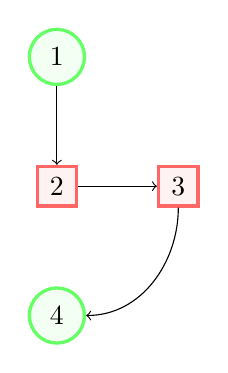
\begin{tikzpicture}[
roundnode/.style={circle, draw=green!60, fill=green!5, very thick, minimum size=7mm},
squarednode/.style={rectangle, draw=red!60, fill=red!5, very thick, minimum size=5mm},
]
%Nodes
\node[squarednode]      (maintopic)                              {2};
\node[roundnode]        (uppercircle)       [above=of maintopic] {1};
\node[squarednode]      (rightsquare)       [right=of maintopic] {3};
\node[roundnode]        (lowercircle)       [below=of maintopic] {4};

%Lines
\draw[->] (uppercircle.south) -- (maintopic.north);
\draw[->] (maintopic.east) -- (rightsquare.west);
\draw[->] (rightsquare.south) .. controls +(down:7mm) and +(right:7mm) .. (lowercircle.east);
\end{tikzpicture}

\end{frame}

\begin{frame}[fragile]

\begin{verbatim}
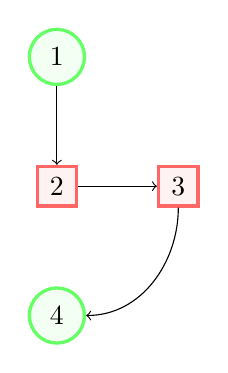
\begin{tikzpicture}[
roundnode/.style={circle, draw=green!60,
fill=green!5, very thick, minimum size=7mm},
squarednode/.style={rectangle, draw=red!60,
fill=red!5, very thick, minimum size=5mm},
]
%Nodes
\node[squarednode] (maintopic)                         {2};
\node[roundnode]   (uppercircle)  [above=of maintopic] {1};
\node[squarednode] (rightsquare)  [right=of maintopic] {3};
\node[roundnode]   (lowercircle)  [below=of maintopic] {4};

%Lines
\draw[->] (uppercircle.south) -- (maintopic.north);
\draw[->] (maintopic.east) -- (rightsquare.west);
\draw[->] (rightsquare.south) .. controls +(down:7mm) 
and +(right:7mm) .. (lowercircle.east);
\end{tikzpicture}
\end{verbatim}

\end{frame}

\begin{frame}
\frametitle{Diagram Recreation Minichallenge}

\url{https://tinyurl.com/dal-latex-challenge-5}

\end{frame}

\begin{frame}[fragile]
\frametitle{Typesetting Plots}

Why shouldn't I just use matplotlib? 
\begin{itemize}
    \item Maintenance
    \item Aesthetics
\end{itemize}

\begin{verbatim}
\usepackage[margin=0.25in]{geometry}
\usepackage{pgfplots}
\pgfplotsset{width=10cm,compat=1.9}

% We will externalize the figures
\usepgfplotslibrary{external}
\tikzexternalize
...
\begin{tikzpicture}
\begin{axis}
\addplot[color=red]{exp(x)};
\end{axis}
\end{tikzpicture}
\end{verbatim}
\end{frame}

\begin{frame}[fragile]
%Here begins the 2D plot
\begin{tikzpicture}
\begin{axis}
\addplot[color=red]{exp(x)};
\end{axis}
\end{tikzpicture}
%Here ends the 2D plot

\end{frame}
\begin{frame}[fragile]
\frametitle{3d plots}

\begin{verbatim}
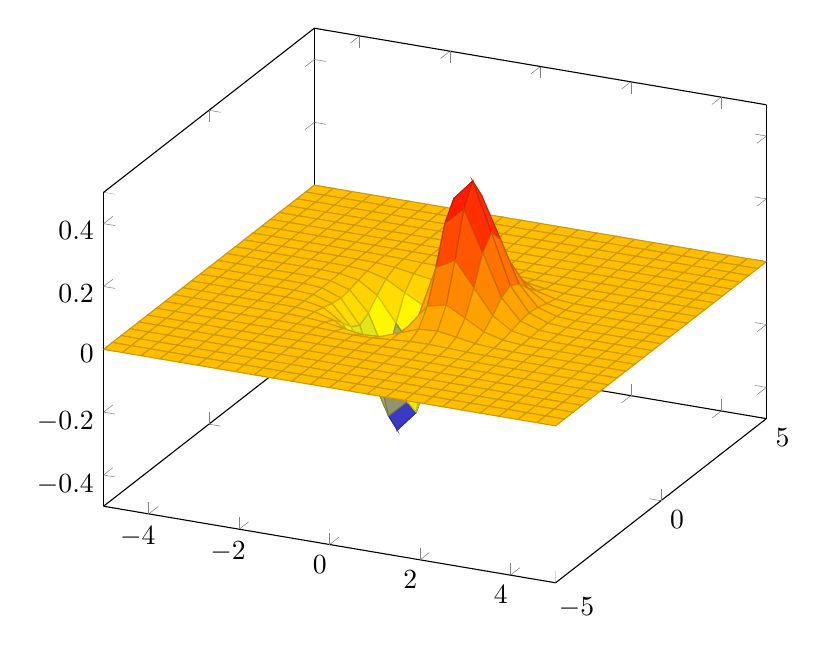
\begin{tikzpicture}
\begin{axis}
\addplot3[
    surf,
]
{exp(-x^2-y^2)*x};
\end{axis}
\end{tikzpicture}
\end{verbatim}

\end{frame}
\begin{frame}[fragile]

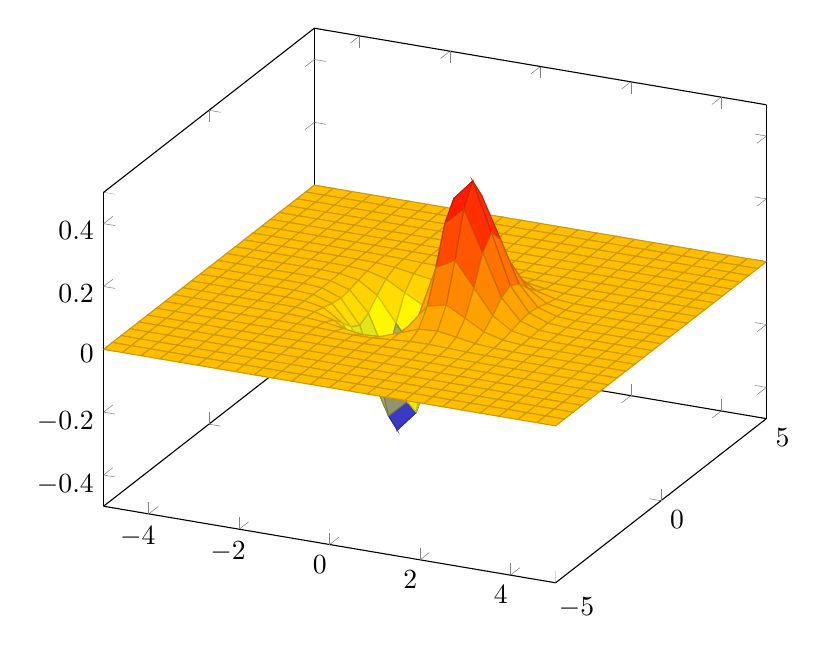
\begin{tikzpicture}
\begin{axis}
\addplot3[
    surf,
]
{exp(-x^2-y^2)*x};
\end{axis}
\end{tikzpicture}

\end{frame}

\begin{frame}[fragile]
\frametitle{Plotting Data}

\begin{verbatim}
\begin{tikzpicture}
    \begin{axis}
    \addplot 
    coordinates {
        (1,2) (2,3) (3,5) (4,6) (5,8) (6,9) (7,10) (8,12)
    };
    \end{axis}
\end{tikzpicture}
\end{verbatim}

\end{frame}
\begin{frame}[fragile]

\begin{tikzpicture}
    \begin{axis}
    \addplot 
    coordinates {
        (1,2) (2,3) (3,5) (4,6) (5,8) (6,9) (7,10) (8,12)
    };
    \end{axis}
\end{tikzpicture}

\end{frame}


\begin{frame}


\frametitle{Plot Recreation Minichallenge}

Link: \url{https://tinyurl.com/dal-latex-challenge-6} \\

\textbf{See:} \url{https://latexdraw.com/} for comprehensive tutorials on latex plotting and diagramming.

\end{frame}

\begin{frame}
\frametitle{\LaTeX Ecosystem}

\begin{itemize}
    \item Presentations (like this one): Beamer
    \item Posers: Beamerposter 
    \item Other documents: overleaf temapltes
    \item Bibliography management: Bibtex, Natbib, Biblatex
    \item Other Packages: \TeX{} Packages
\end{itemize}


\textbf{Dal Specific:} There is a Dal poster template on overleaf (if you search), I made a Dal presentation template (ask me), Vlado and Mike maintain the thesis template: \url{https://web.cs.dal.ca/~vlado/dalcsthesis/}. There are other things (RAD templates) others have maintained.

\end{frame}

\begin{frame}[fragile]
\frametitle{Citations and References}

\begin{verbatim}
\usepackage{natbib}
\bibliographystyle{unsrtnat}
...
\section{My Paper}
According to \citet{} ....
This has been studied by many works \citep{}.
Our results differ (see \citealp{})...
...
\bibliography{bibliography}
\end{verbatim}

\texttt{bibliography.bib}
\begin{verbatim}
@misc{knuthwebsite,
    author    = "Donald Knuth",
    title     = "Knuth: Computers and Typesetting",
    url       = "http://www-cs-faculty.stanford.edu/\~{}uno/abcde.html"
}
\end{verbatim}
\end{frame}
\begin{frame}[fragile]
\frametitle{Citation flow demo}

\textbf{get paper bibtex from semantic scholar}

\end{frame}

\begin{frame}[fragile]
\frametitle{Citation Styles}

\textbf{There are various citation}: packages like bibtex, biblatex, natbib
\vfill
You will need to be careful when setting the bibliography, bibliography style, citations, and bibtex entries.
\vfill
\textbf{Bibtex Entries}
\url{https://www.bibtex.com/e/entry-types/} \\
Common mistake: using @misc when @article is available.
\vfill
\textbf{When to use citep/citet/citealp/cite}
If your citation style supports it you should use \verb|\citep| when its a parenthesis citation and you are not directly referring to the citation as a noun. If you using the citation as a noun, use \verb|citet|. Avoid extra parenthesis in a parenthesis by using \verb|\citealp|.
\vfill
Do not refer to a \verb|\cite| directly. ``[1] shows blah.'' Instead say "Lou et al. [1] shows blah.

\end{frame}

\begin{frame}[fragile]
\frametitle{Advanced \LaTeX}

\begin{itemize}
    \item Stylesheets
    \item Macros, Commands 
    \item Large scale documents
    \item Tikz, Pgfplots
\end{itemize}

\begin{verbatim}
\newcommand{\R}{\mathbb{R}} 
\newcommand{\bb}[1] {\mathbb{#1}}
\( \bb{R} \) 
\end{verbatim}

\end{frame}



\begin{frame}
\frametitle{Additional Learning Resources}

\begin{enumerate}
    \item Overleaf
    \item \url{https://www.youtube.com/@DrTrefor}
    \item Looking at the source of arXiv papers
    \item \url{https://texnique.xyz/}
    \item Michelle Krummel Latex Youtube
    \item Me / Other Grad students at Dal
    \item \url{https://www.learnlatex.org/en/}
\end{enumerate}

\end{frame}
\begin{frame}
\frametitle{Competition}

Paper recreation challenge (1 hour)
\vfill
\begin{enumerate}
    \item Choose a paper from the TinyPapers track from ICRL: \url{https://tinyurl.com/dal-latex-tiny-papers}
    \item Create a new overleaf project using the ICLR template \url{https://tinyurl.com/dal-latex-iclr-template}
    \item Fill it in copying the paper as best you can.
\end{enumerate}
\vfill
\textbf{The most faithful and challenging recreation wins! Judged by Frank and I}
\vfill
\textbf{Submit to domenic.rosati@dal.ca}

\end{frame}


\begin{frame}
\frametitle{Competition}

The most faithful and challenging recreation wins!
\vfill
What is allowed?
\begin{itemize}
    \item Taking screenshots of figures and diagrams
    \item Looking things up
    \item Asking for help
\end{itemize}
\vfill
What is not allowed?
\begin{itemize}
\item Finding the TeX source of the paper
\item Taking screenshots of tables (they should be tables)
\end{itemize}
\vfill
\textbf{Ask for help!}
\vfill
\textbf{Finished?}
\url{https://texnique.xyz/}

\end{frame}



\begin{frame}
\frametitle{References}

\printbibliography

\end{frame}
\end{document}